\documentclass{beamer}
%\documentclass[aspectratio=169]{beamer}
%
\mode<presentation>
{
  \usetheme{default}      
  \usecolortheme{default}
  \usefonttheme{default} 
  \setbeamertemplate{navigation symbols}{}
  \setbeamertemplate{caption}[numbered]
} 

\usepackage[english]{babel}
\usepackage[utf8x]{inputenc}
\usepackage{pgfplots}
\pgfplotsset{compat=1.12}

\newcommand{\norm}[1]{\left\lVert#1\right\rVert}

\title[Classification]{Introduction to Machine Learning}
\subtitle{Lecture 4: Clustering}
\author{Alexis Zubiolo\newline\texttt{alexis.zubiolo@gmail.com}}
\institute{Data Science Team Lead @ Adcash}
\date{\today}

\begin{document}

\begin{frame}
  \titlepage
\end{frame}

\begin{frame}{What is clustering?}
\textbf{Clustering} algorithms aim at \textbf{grouping unlabeled objects}.
\vfill
\pause
\textbf{Goal}: Find clusters such that objects in the same cluster are more similar to each other than to objects in other clusters.
\pause
\vfill
Main challenges:
\begin{itemize}
	\item What does \textit{similar} mean?
	\item Given a similarity definition, how do we define clusters?
	\item How many clusters?
\end{itemize}
\end{frame}

\begin{frame}
	\center \Huge{$k$-means}
\end{frame}

\begin{frame}{$k$-means}
Split the set of points into $k$ classes.

\end{frame}

\begin{frame}{$k$-means}

We look for a partition $S = \left\{ S_1, S_2, \dots, S_k\right\}$ minimizing the within-cluster sum of squares.
\begin{equation*}
\arg \min_S \sum_{i = 1}^{k} \sum_{x \in S_i} \norm{x - \mu_i}_2^2
\end{equation*}
where 
\begin{equation*}
\mu_i = \dfrac{1}{|S_i|} \sum_{x \in S_i} x
\end{equation*}
is the mean of points in $S_i$.
\end{frame}

\begin{frame}{$k$-means}
\textbf{Remark}: The $k$-means solution depends on the initial position of the $\mu_i$s centroids.

(see animation by Andrey Shabalin)
\vfill
\pause
2 related questions:
\begin{enumerate}
	\item How to choose the initial $\mu_i$s?
	\item How to have more stable results?
\end{enumerate}
\vfill
\pause
Unfortunately, no miracle strategy for Q1. A common strategy:
\begin{itemize}
	\item Several $k$-means with random initializations
	\item Majority vote
\end{itemize}
\end{frame}

\begin{frame}
\begin{center}
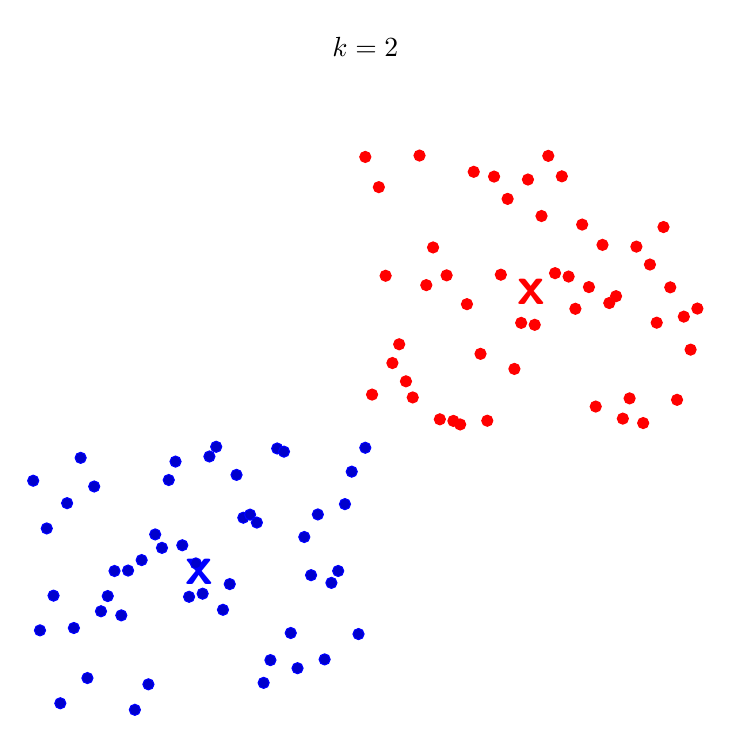
\begin{tikzpicture}
  \begin{axis}[
        width=\linewidth,
        title={$k=2$},
        hide axis,
        xmin=0,xmax=10,ymin=0,ymax=100,
        xlabel={$x_1$},
        ylabel={$x_2$}
        ]
       \node[text=blue,font=\sffamily\bfseries,scale=2] at (3,30) {x};
       \addplot+[y filter/.expression={y+10},only marks,mark=*,samples=50,domain=1:5] {40*rnd};
       \node[text=red,font=\sffamily\bfseries,scale=2] at (7,70){x};
       \addplot+[y filter/.expression={y+50},only marks,mark=*,mark options={fill=red},samples=50,domain=5:9] {40*rnd};
  \end{axis}
\end{tikzpicture}
\end{center}
\end{frame}

\begin{frame}{Speeding up $k$-means}
Each $k$-means iteration iterates over all the points in the dataset. This can be computationally expensive, especially if
\begin{itemize}
	\item There are many points
	\item The point density is big
\end{itemize}
What to do to speed up the process?
\pause
\vfill
\textbf{Alternative}: \textbf{Mini-batch} $k$-means. At each iteration
\begin{itemize}
	\item Choose a subset of points
	\item Apply a $k$-means iteration 
\end{itemize}
\end{frame}

\begin{frame}{Number of clusters}
In some applications, you know how many clusters you want. In this case, $k$ is \textbf{easy to set}.
\vfill
In other applications, we don't know the optimal number of classes we want. Ideally, we would like $k$ to be selected automatically.
\vfill
There is always some ambiguity in selection the \textit{optimal} number of clusters. This is normal: When doing unsupervised learning, there is necessarily some inherent subjectivity in the labeling process!
\end{frame}

\begin{frame}{Number of clusters}
That being said, it is possible to define some criterias to determine whether $k_1$ is a better number of clusters than $k_2$. We can use the sum of squared errors to the centroids:
\begin{equation*}
\text{SSE}(k) = \sum_{i = 1}^{k} \sum_{x \in S_i} \norm{x - \mu_i}_2^2
\end{equation*}
And apply the \textbf{Elbow method}.
\vfill
\pause
Note that this is not a miracle solution.
\end{frame}

\begin{frame}
	\center \Huge{Hierarchical clustering}
\end{frame}

\begin{frame}{Hierarchical clustering}


But then, which partition do we use?
\end{frame}

\begin{frame}{Hierarchical clustering: Dendograms}
\begin{tikzpicture}[sloped]
\node (a) at (-6,0) {a};
\node (b) at (-3,0) {b};
\node (c) at (-0.5,0) {c};
\node (d) at (0.5,0) {d};
\node (e) at (2,0) {e};
\node (ab) at (-4.5,3) {};
\node (cd) at (0,1) {};
\node (cde) at (1,2) {};
\node (all) at (-1.5,5) {};

\draw  (a) |- (ab.center);
\draw  (b) |- (ab.center);
\draw  (c) |- (cd.center);
\draw  (d) |- (cd.center);
\draw  (e) |- (cde.center);
\draw  (cd.center) |- (cde.center);
\draw  (ab.center) |- (all.center);
\draw  (cde.center) |- (all.center);

\pause
\draw[dashed, thick, red] (-6.5,2.5) -- (+2.5,+2.5);
\pause
\draw[dashed, thick, blue] (-6.5,3.5) -- (+2.5,+3.5);
\pause
\draw[->] (-7,0) -- node[above]{distance} (-7,6);
\pause
\draw[<-] (+3,0) -- node[below]{number of clusters} (+3,6);
\end{tikzpicture}
\end{frame}

\begin{frame}{Hierarchical clustering, pros \& cons}

\end{frame}

\begin{frame}{Conclusion}
Clustering methods create groups of unlabeled points.
\vfill
\pause
They rely on:
\begin{itemize}
	\item A similarity measure (\textit{e.g.} the Euclidian norm)
	\item A few parameters, \textit{e.g.}
	\begin{itemize}
		\item The number of clusters for $k$-means
		\item The dendogram cut for hierarchical clustering
	\end{itemize}
\end{itemize}
\vfill
\pause
Clusters can be represented by a dendogram.
\end{frame}

\begin{frame}
	\center
	\huge{Thank you! Questions}
\end{frame}

\end{document}